\graphicspath{{chapters/5.Chapter_3/figures}}

\chapter{Transporters}

http://hallam.microbiology.ubc.ca/MetaPathways/

\section{Introduction}

\section{Aims}

The principal aim of this chapter is to identify
transporter proteins present in the host and endosymbiont
binned transcripts from the CCAP1660/12 RNA-Seq analysis,
a re-assembly of the \citep{Kodama2014c} dataset.

Finally, this will be compared with the 
endosymbiont 


\section{Methods}

\subsection{Data Acquisition}

Sets of algal predicted proteins were acquired as follows:

\subsubsection{\textit{Chlorella variabilis} NC64A and \textit{Coccomyxa subellipsoidea} C-169} 
 
\textit{Coccomyxa subellipsoidea} C-169 genome project \citep{Blanc2012} version 2.0 
JGI annotated proteins (created 12-01-2014) were downloaded from JGI's
Phyotozome v10.3.1 \citep{Goodstein2012}. 
Similarly, the ``best'' annotated proteins from
version 1 of the \textit{Chlorella variabilis} NC64A genome project \citep{Blanc2010}
were downloaded from JGI's genome portal \citep{Grigoriev2011,Nordberg2014}

\subsubsection{\textit{Micractinium reisseri}}

Sequences were derived from endosymbiont binned
transcripts and annotations as described in \ref{chap:transcriptomics}.




\subsubsection{\textit{Chlorella variabilis 1 N}}

\(232.3M\) 100bp paired-end reads from \citep{Kodama2014}'s 
bulk RNAseq transcriptome of \textit{Paramecium bursaria} Yad1g (syngen
3, mating type 1) bearing \textit{Chlorella variabilis} 1N endosymbionts
were downloaded from the DNA Data Bank of Japan (DDBJ) \citep{Tateno2002,Kaminuma2011}
in Sequence Read Archive (SRA) format \citep{Leinonen2011,KodamaNRA2012b}. 

These reads were then converted to fastq using ``fastq-dump'' using the SRA Toolkit
\citep{NationalCenterforBiotechnologyInformation2011}.  Reads were then trimmed
for sequencing adapters using ILLUMINACLIP and SLIDINGWINDOW with a window size
of 4 and a minimum average quality of 30.














sequencing


DDBJ Sequence Read Archive (DRA) (accession number DRA000907, http://trace.ddbj.nig.ac.jp/DRASearch/submission?acc=DRA000907



\subsection{Transporter Identification}

\subsection{qPCR}


\section{Results}


\subsection{Kodama Assembly}


SUMMARY OF KODAMA ASSEMBLY PARAMETERS
AND BINNING SIZES


\subsubsection{Assembly}

Mapping to assembly

\begin{figure}
	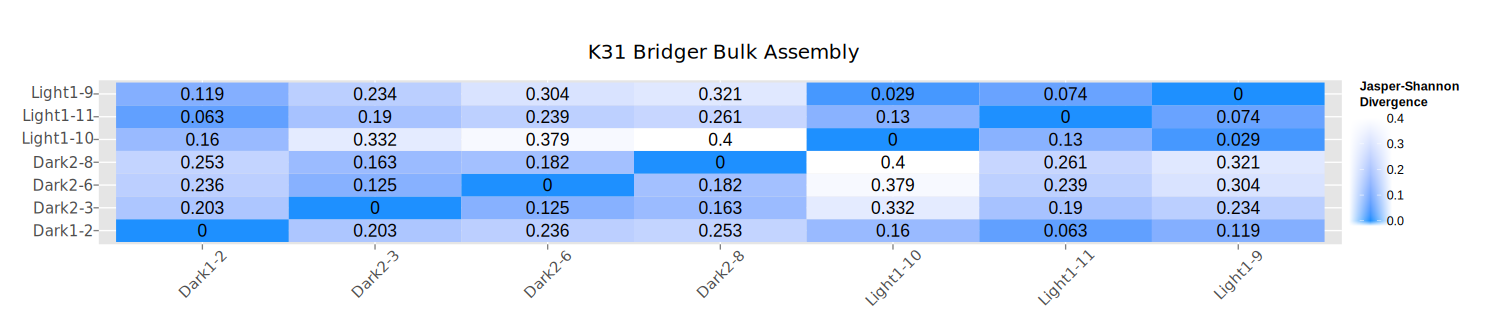
\includegraphics{bridger_bulk_only_sct_kallisto_mapping_jsd.pdf}[width=\textwidth]
	\caption{SCT sample-wise similarities - entire libraries post trimming
		no error correction or normalisation mapped to a Bridger transcriptome 
		assembly of an error corrected, digitally normalised Bulk Assembly.  
		This was conducted to check whether similarities between samples
		were being biased by something?}
	\label{fig:bridger_bulk_heatmap}
\end{figure}




\subsection{Kallisto quantification analysis}





\subsection{Transporter identification}

To identify transporters present in the translated protein dataset of the 
endosymbiont bins of the CCAP1660/12 and YADGN1 
\textit{Paramecium bursaria} transcriptome assemblies, as well as the Chlorella NC64A 
and Coccoymxa C-169 predicted proteomes the following process was used:

\begin{enumerate}
        \item TMHMM was used to predict TM domains within each protein
        \item Proteins were then filtered on those of which had 3 or more TM domains
        \item Those proteins were then searched using HMM and the PFAM HMM database
        \item Those hits were parsed for those which shared a PFAM domain with TCDB proteins
\end{enumerate}

\subsection{Quantification}



\section{Discussion}

\subsection{Quantification in MDA}
\\


%Titrating ERCC spike-ins to level of single cell 
%It has become an increasingly established methodology to add RNA of known concentrations
%to extractions before library preparation to aid quantification
%and normalisation in downstream analysis. 
%Unforunately, there are no established methods for synthetic RNA spike-ins
%of known RNA concentrations (e.g. ERCC RNA standards \citep{Jiang2011}) with MDA
%sc-RNAseq. Specifically, standards would need to be carefully titrated to appropriate
%concentrations for single cell methods or they would overwhelm sequencing 


%therefore no such spike-ins were added. 

%    \item Just use SCT for transcript quantification i.e. map the SCT reads to a bulk derived \textit{de novo} assembly to generate counts (and is there a severe bias induced 
%        by the MDA amplification \citep{Liang2014}?)
%\end{itemize}  <>++
%However, MDA is prone to a degree of amplification bias \citep{Liang2014} which may be problematic in accurate inference of differential expression
%therefore, the suitability of MDA-based scRNA-Seq in particular will also need to be assessed.
%The only other published analysis of \textit{Paramecium bursaria} and its green algal endosymbionts by \citep{Kodama2014} largely
%side-stepped this issue by focussing on the analysis of host transcripts with and without the endosymbiont by filtering
%likely endosymbiont derived contigs from analysis using a crude MEGABLAST \(e^{-40}\) approach.
%Studies in related ciliates have demonstrated a high prevalence of alternative splicing events (5.2\% of genes in \textit{Tetrahymena
%    thermophila} for a single celled eukaryote \citep{Xiong2012}
%This paper also demonstrated the huge dynamic range of expression (and thus necessity of RNA-Seq over microarray approaches) in \textit{T. thermophila})
%with approximately 6 order of magnitude range \citep{Xiong2012}
%However, as both target species - host and endosymbiont are eukaryotes the complication of mRNA enrichment 
%is simplified due to the sufficiency of poly-A selection for this task (instead of rRNA depletion methods)
%Determining the necessary sequencing depth is also difficult.
%First achieved in \citep{Lao2009}



SPIKEINS - needed to control statistical noise Kim2015

chimera analysis


MDA has amplification bias with GC content - problem for PbMr \citep{Macaulay2014}



\section{Conclusion}


Network analysis
http://www.ncbi.nlm.nih.gov/pmc/articles/PMC3299011/pdf/fmicb-03-00085.pdf



%Genome assembly - spades macmanes trimming was worse than spades harash trimming (shorter contigs)
